% Options for packages loaded elsewhere
\PassOptionsToPackage{unicode}{hyperref}
\PassOptionsToPackage{hyphens}{url}
%
\documentclass[
  a4paper,
]{article}
\usepackage{amsmath,amssymb}
\usepackage{setspace}
\usepackage{iftex}
\ifPDFTeX
  \usepackage[T1]{fontenc}
  \usepackage[utf8]{inputenc}
  \usepackage{textcomp} % provide euro and other symbols
\else % if luatex or xetex
  \usepackage{unicode-math} % this also loads fontspec
  \defaultfontfeatures{Scale=MatchLowercase}
  \defaultfontfeatures[\rmfamily]{Ligatures=TeX,Scale=1}
\fi
\usepackage{lmodern}
\ifPDFTeX\else
  % xetex/luatex font selection
\fi
% Use upquote if available, for straight quotes in verbatim environments
\IfFileExists{upquote.sty}{\usepackage{upquote}}{}
\IfFileExists{microtype.sty}{% use microtype if available
  \usepackage[]{microtype}
  \UseMicrotypeSet[protrusion]{basicmath} % disable protrusion for tt fonts
}{}
\makeatletter
\@ifundefined{KOMAClassName}{% if non-KOMA class
  \IfFileExists{parskip.sty}{%
    \usepackage{parskip}
  }{% else
    \setlength{\parindent}{0pt}
    \setlength{\parskip}{6pt plus 2pt minus 1pt}}
}{% if KOMA class
  \KOMAoptions{parskip=half}}
\makeatother
\usepackage{xcolor}
\usepackage[margin=1in]{geometry}
\usepackage{color}
\usepackage{fancyvrb}
\newcommand{\VerbBar}{|}
\newcommand{\VERB}{\Verb[commandchars=\\\{\}]}
\DefineVerbatimEnvironment{Highlighting}{Verbatim}{commandchars=\\\{\}}
% Add ',fontsize=\small' for more characters per line
\usepackage{framed}
\definecolor{shadecolor}{RGB}{248,248,248}
\newenvironment{Shaded}{\begin{snugshade}}{\end{snugshade}}
\newcommand{\AlertTok}[1]{\textcolor[rgb]{0.94,0.16,0.16}{#1}}
\newcommand{\AnnotationTok}[1]{\textcolor[rgb]{0.56,0.35,0.01}{\textbf{\textit{#1}}}}
\newcommand{\AttributeTok}[1]{\textcolor[rgb]{0.13,0.29,0.53}{#1}}
\newcommand{\BaseNTok}[1]{\textcolor[rgb]{0.00,0.00,0.81}{#1}}
\newcommand{\BuiltInTok}[1]{#1}
\newcommand{\CharTok}[1]{\textcolor[rgb]{0.31,0.60,0.02}{#1}}
\newcommand{\CommentTok}[1]{\textcolor[rgb]{0.56,0.35,0.01}{\textit{#1}}}
\newcommand{\CommentVarTok}[1]{\textcolor[rgb]{0.56,0.35,0.01}{\textbf{\textit{#1}}}}
\newcommand{\ConstantTok}[1]{\textcolor[rgb]{0.56,0.35,0.01}{#1}}
\newcommand{\ControlFlowTok}[1]{\textcolor[rgb]{0.13,0.29,0.53}{\textbf{#1}}}
\newcommand{\DataTypeTok}[1]{\textcolor[rgb]{0.13,0.29,0.53}{#1}}
\newcommand{\DecValTok}[1]{\textcolor[rgb]{0.00,0.00,0.81}{#1}}
\newcommand{\DocumentationTok}[1]{\textcolor[rgb]{0.56,0.35,0.01}{\textbf{\textit{#1}}}}
\newcommand{\ErrorTok}[1]{\textcolor[rgb]{0.64,0.00,0.00}{\textbf{#1}}}
\newcommand{\ExtensionTok}[1]{#1}
\newcommand{\FloatTok}[1]{\textcolor[rgb]{0.00,0.00,0.81}{#1}}
\newcommand{\FunctionTok}[1]{\textcolor[rgb]{0.13,0.29,0.53}{\textbf{#1}}}
\newcommand{\ImportTok}[1]{#1}
\newcommand{\InformationTok}[1]{\textcolor[rgb]{0.56,0.35,0.01}{\textbf{\textit{#1}}}}
\newcommand{\KeywordTok}[1]{\textcolor[rgb]{0.13,0.29,0.53}{\textbf{#1}}}
\newcommand{\NormalTok}[1]{#1}
\newcommand{\OperatorTok}[1]{\textcolor[rgb]{0.81,0.36,0.00}{\textbf{#1}}}
\newcommand{\OtherTok}[1]{\textcolor[rgb]{0.56,0.35,0.01}{#1}}
\newcommand{\PreprocessorTok}[1]{\textcolor[rgb]{0.56,0.35,0.01}{\textit{#1}}}
\newcommand{\RegionMarkerTok}[1]{#1}
\newcommand{\SpecialCharTok}[1]{\textcolor[rgb]{0.81,0.36,0.00}{\textbf{#1}}}
\newcommand{\SpecialStringTok}[1]{\textcolor[rgb]{0.31,0.60,0.02}{#1}}
\newcommand{\StringTok}[1]{\textcolor[rgb]{0.31,0.60,0.02}{#1}}
\newcommand{\VariableTok}[1]{\textcolor[rgb]{0.00,0.00,0.00}{#1}}
\newcommand{\VerbatimStringTok}[1]{\textcolor[rgb]{0.31,0.60,0.02}{#1}}
\newcommand{\WarningTok}[1]{\textcolor[rgb]{0.56,0.35,0.01}{\textbf{\textit{#1}}}}
\usepackage{graphicx}
\makeatletter
\def\maxwidth{\ifdim\Gin@nat@width>\linewidth\linewidth\else\Gin@nat@width\fi}
\def\maxheight{\ifdim\Gin@nat@height>\textheight\textheight\else\Gin@nat@height\fi}
\makeatother
% Scale images if necessary, so that they will not overflow the page
% margins by default, and it is still possible to overwrite the defaults
% using explicit options in \includegraphics[width, height, ...]{}
\setkeys{Gin}{width=\maxwidth,height=\maxheight,keepaspectratio}
% Set default figure placement to htbp
\makeatletter
\def\fps@figure{htbp}
\makeatother
\setlength{\emergencystretch}{3em} % prevent overfull lines
\providecommand{\tightlist}{%
  \setlength{\itemsep}{0pt}\setlength{\parskip}{0pt}}
\setcounter{secnumdepth}{-\maxdimen} % remove section numbering
\ifLuaTeX
\usepackage[bidi=basic]{babel}
\else
\usepackage[bidi=default]{babel}
\fi
\babelprovide[main,import]{catalan}
% get rid of language-specific shorthands (see #6817):
\let\LanguageShortHands\languageshorthands
\def\languageshorthands#1{}
\ifLuaTeX
  \usepackage{selnolig}  % disable illegal ligatures
\fi
\usepackage{bookmark}
\IfFileExists{xurl.sty}{\usepackage{xurl}}{} % add URL line breaks if available
\urlstyle{same}
\hypersetup{
  pdftitle={U2. Windows Server. Instal·lació i ús (II)},
  pdfauthor={@tofermos 2024},
  pdflang={ca-ES},
  hidelinks,
  pdfcreator={LaTeX via pandoc}}

\title{U2. Windows Server. Instal·lació i ús (II)}
\author{@tofermos 2024}
\date{}

\begin{document}
\maketitle

{
\setcounter{tocdepth}{2}
\tableofcontents
}
\setstretch{1.5}
\newpage
\renewcommand\tablename{Tabla}

\section{1 Resum}\label{resum}

En aquesta unitat prèvia a la creació d'un domini:

\begin{enumerate}
\def\labelenumi{\arabic{enumi}.}
\item
  Configurarem les MV com a Xarxa Interna. Emulem una xarxa local de
  computadores connectades a un switch.
\item
  Configurarem la xarxa Windows mitjançant IP fixes privades en la
  mateixa xarxa.
\item
  Coneixerem sobre protocols i Firewall :
\end{enumerate}

\begin{itemize}
\tightlist
\item
  protocols i aplicacions (detecció de xarxes i compartició en Windows)
\item
  altres prrotocols com el ICMP4 (ping) o SMB
\item
  les restriccions del Firewall
\end{itemize}

\begin{enumerate}
\def\labelenumi{\arabic{enumi}.}
\setcounter{enumi}{3}
\item
  Estudiarem aspectes bàsics de la compartició de carpetes.
\item
  Treballarem la captura d'unitats (GUI/CLI)
\item
  Veurem algunes configuracions generals simples ( nom del PC i WG,
  Actualizacions automàtiques, Zona horària\ldots)
\end{enumerate}

\section{2 Canviar el nom del servidor i
Workgroup}\label{canviar-el-nom-del-servidor-i-workgroup}

\begin{figure}
\centering
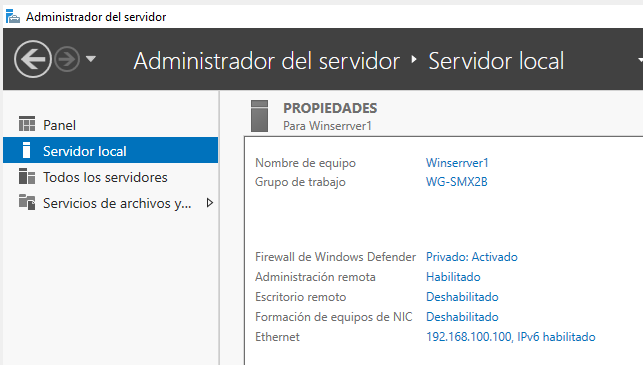
\includegraphics{png/ADDS/WorkgroupNomEquip.png}
\caption{\emph{Figura1: Nom equip i del Grup de Treball}}
\end{figure}

Configurar la xarxa Servidor

\section{3 Configuració de la xarxa en Virtualbox. ``Xarxa
Interna''}\label{configuraciuxf3-de-la-xarxa-en-virtualbox.-xarxa-interna}

Estem ``conectant cables al switch''.

De moment només ens fa falta la tarja que es connectarà a un switch on
es conecten la resta de PC de la xarxa () ``xarxa interna'').

Podem instal·lar un segon adaptador per disposar de la connexió
d'Internet de l'amfitrió (adaptador NAT). De moment és opcional.

\begin{figure}
\centering
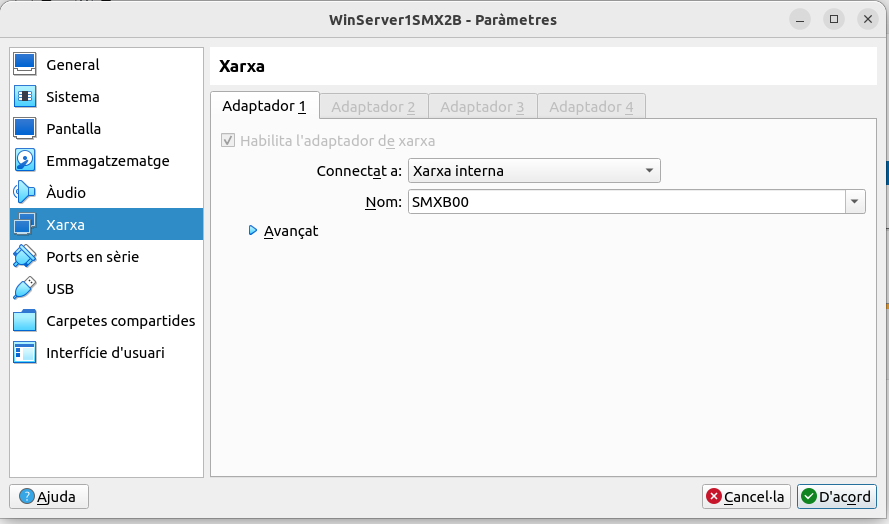
\includegraphics{png/ADDS/xarxainterna.png}
\caption{\emph{Figura 2: Xarxa interna}}
\end{figure}

\begin{quote}
NOTA:

En el WINDOWS 1x hem de tindre NOMÉS la tarja interna. No perdeu de
vista la ``realitat'' que estem emulant !
\end{quote}

\section{4 Configuració de la xarxa en
Windows.}\label{configuraciuxf3-de-la-xarxa-en-windows.}

\subsection{4.1 Firewall de Windows. Aplicaciones
permitidas}\label{firewall-de-windows.-aplicaciones-permitidas}

Des del mateix Administrador de Servidor accedir al \textbf{Firewall:
Aplicaciones permitidas} i assegurar que ens permeta Compartir i
Detectar recursos a través de la xarxa. Dos capacitat que activarem en
l'apartat següent:

\begin{figure}
\centering
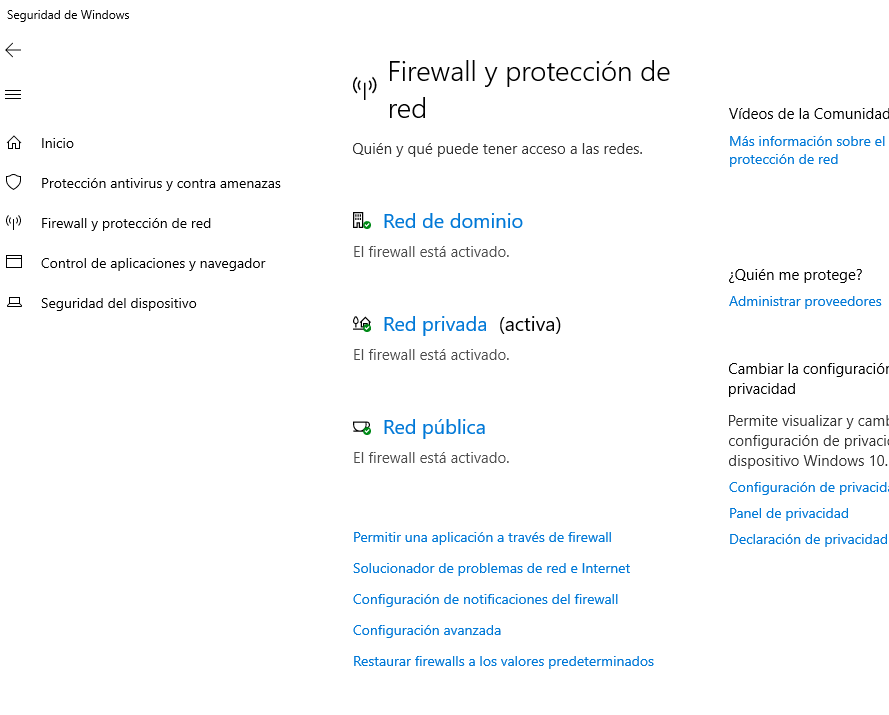
\includegraphics{png/ADDS/PermitirUnaAplicacionATravesdeFirewall.png}
\caption{\emph{Figura 3: Permitir una aplicación a través de Firewall}}
\end{figure}

\begin{figure}
\centering
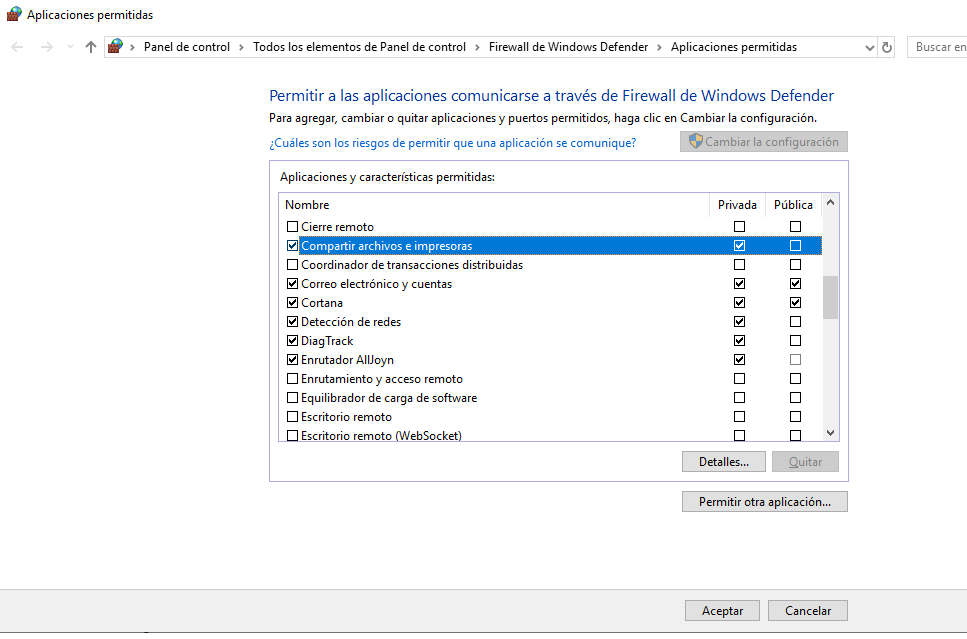
\includegraphics{png/ADDS/FirewallCompartiryDetectar.png}
\caption{\emph{Figura 4: Firewall permet compartir y detectar xarxes}}
\end{figure}

`

\subsection{4.2 IPs privades en la mateixa
xarxa}\label{ips-privades-en-la-mateixa-xarxa}

Com ja sabeu del mòdul de XAL de 1r de SMX haureu de configurar les IPs.
Per exemple:

IP Windows 1X: 192.168.0.2/24\\
IP Windows Server: 192.168.0.1/24

\emph{Windows+R: Configuración, Red e internet, Centro de Redes y
Recursos Compartidos, Ethernet}

\begin{figure}
\centering
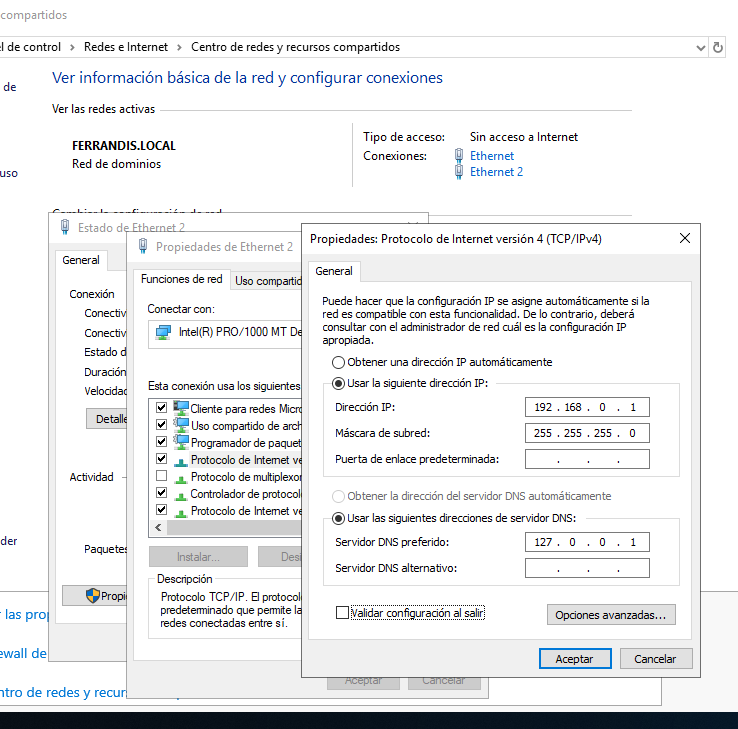
\includegraphics{png/ADDS/tarja2.png}
\caption{\emph{Figura 5: Adaptador de xarxa}}
\end{figure}

\subsection{4.3 Detecció de xarxes i
recursos}\label{detecciuxf3-de-xarxes-i-recursos}

\emph{Windows+R: Configuración, Red e internet, Centro de Redes y
Recursos Compartidos}

Com ja vam estudiar a la Unitat anterior amb el Wordgroup fet amb PC
Windows 1x, hem d'activar per a las *\textbf{xarxa privada} en totes les
màquines

\begin{itemize}
\item
  Activar la detecció de xarxes
\item
  Activar l'ús compartit de carpetes i impressores.
\end{itemize}

Configuración, Red e internet ( o \emph{Win + I}) Centro de Redes y
Recursos Compartidos, Cambiar configuración del Uso compartido
avanzado:*

\includegraphics{png/ADDS/ActivaDetecciónyUsoCompartidoPrivada.png}

\includegraphics{png/ADDS/ActivaDetecciónyUsoCompartidoPublico.png}

\includegraphics{png/ADDS/ActivaUsoCompartidoCarpetasPúblicasyContrasenya.png}

\subsection{4.4 Problema en Windows Server i la Xarxa
Privada}\label{problema-en-windows-server-i-la-xarxa-privada}

\textbf{Problema:}

En Xarxa Privada, marquem les opcions però quan entrem veiem que estan
desactivades No es detecten les carpetes compartides, ni tant sols els
PCs de la xarxa.

En canvi sí podem accedir a les carpetes mitjançant els comandament
\emph{net use}

\textbf{Raó}:

La detecció de serveis compartits depén d'altres serveis que no estan
executant-se.

\textbf{Solució:}

Abans que res assegureu-vos que teniu el Firewall configurat com hem
indicat al punt anterior (\textbf{Aplicaciones permitidas\ldots{}}). Si
és correcte\ldots{}

Fent spoiler al tema de \textbf{Serveis de Windows} que tractarem més
avant, cal que activem una sèrie de serveis necessaris (dependències)

Alguns d'aquests servicis podrem inciar-los des l'Administrador del
Servidor (\emph{servermanager.exe}) que tenim obert normalment però
altres no. Això es deu a que no estan habilitats, caldrà executar la
consola de microsoft específica de servicis (\emph{services.msc}) i
habilitar-los prèviament.

Els serveis que cal que estiguen executant-se (dependències) són:

\begin{itemize}
\tightlist
\item
  Client DNS
\item
  Publicación de resursos de deteccción de
\item
  Detección host de SSDP
\item
  Dispositivo host de UPnP
\end{itemize}

Per a iniciar els servicis primer cal que estiguen habilitats. Per això
anem a la \textbf{consola MC de servicis} amb \emph{Win R:
services.msc}).

1.- Assegurem que estiguen no estiguen deshabilitats. El tipus d'inici
ha de ser \textbf{Automático} per a que s'engeguen en iniciar el
servidor.

\begin{figure}
\centering
\includegraphics{png/ADDS/ServicioDetecciónSSDP.png}
\caption{\emph{Figura 8: Canviem en tipus d'inici a Automático}}
\end{figure}

2.- Podem iniciar manualment per no reiniciar ara.

\begin{figure}
\centering
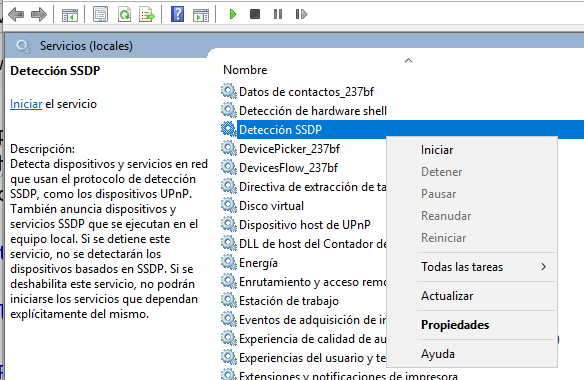
\includegraphics{png/ADDS/ServiciInici.png}
\caption{\emph{Figura 9: Iniciem manuelament un servici}}
\end{figure}

\begin{quote}
Nota:

Encara que supose continuar fent spoiler sobre el tema de servicis,
observa que amb un \textbf{Inici automàtic}, el servei està en marxa en
engegar-se el servidor \textbf{sense necessitat d'iniciar sessió al
Servidor} \#\# 4.5 Provar la connectivitat amb el protocol ICMP (ping)
\end{quote}

Una prova molt clàssica és la del ping (protocol ICMP4). La fem des de
totes les màquines.

\begin{figure}
\centering
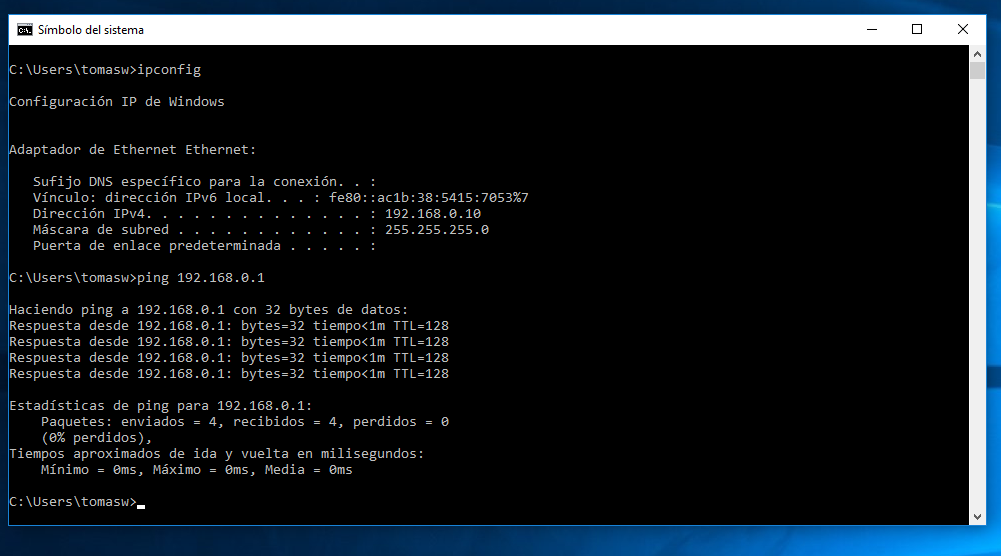
\includegraphics{png/ADDS/ping.png}
\caption{\emph{Ping des de totes les màquines de la xarxa}}
\end{figure}

Si tenim problemes podem revisar, la configuració del Firewall:

!\emph{Firewall ICMP4 (echo
entrada)}{]}(png/ADDS/FirewallICMP4Entrada.png)

\begin{figure}
\centering
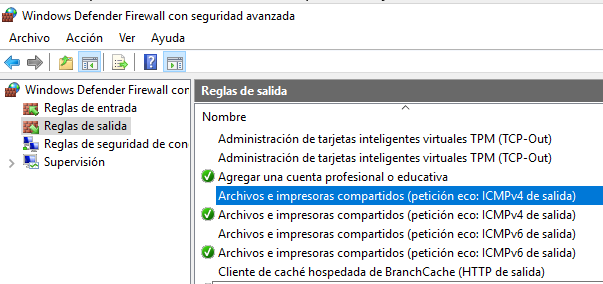
\includegraphics{png/ADDS/FirewallICMP4Salida.png}
\caption{\emph{Firewall ICMP4 (echo salida)}}
\end{figure}

\section{\texorpdfstring{5 Aspectes bàsics de la configuració des del
\emph{msconfig}}{5 Aspectes bàsics de la configuració des del msconfig}}\label{aspectes-buxe0sics-de-la-configuraciuxf3-des-del-msconfig}

Un exemple podria ser desactivar/activar el \textbf{Servei
d'actualitzacions}

\begin{quote}
Nota sobre les actualitzacoins automàtiques

És important que entengueu el que pot suposar tindre activada esta opció
en un servidor real aplicacions i middleware instal·lat i molts clients
depenent-ne.
\end{quote}

\emph{Win + R: msconfig.exe}

Altre exemple podria ser assegurar la \textbf{Zona horària}.

Cal connexió a Internet. Caldrà una segona tarja connectada a un router
(NAT en l'emulació nostra de Virtualbox)

\section{6 Recursos compartits en
xarxa}\label{recursos-compartits-en-xarxa}

\subsection{6.1 Compartició de
carpetes}\label{comparticiuxf3-de-carpetes}

La compartició de carpetes la farem sense especificar permisos per a
usuaris donat que encra no tenim ususari del domini. No anem a
``replicar-los'' com hem fet en un Workgroup.

\begin{figure}
\centering
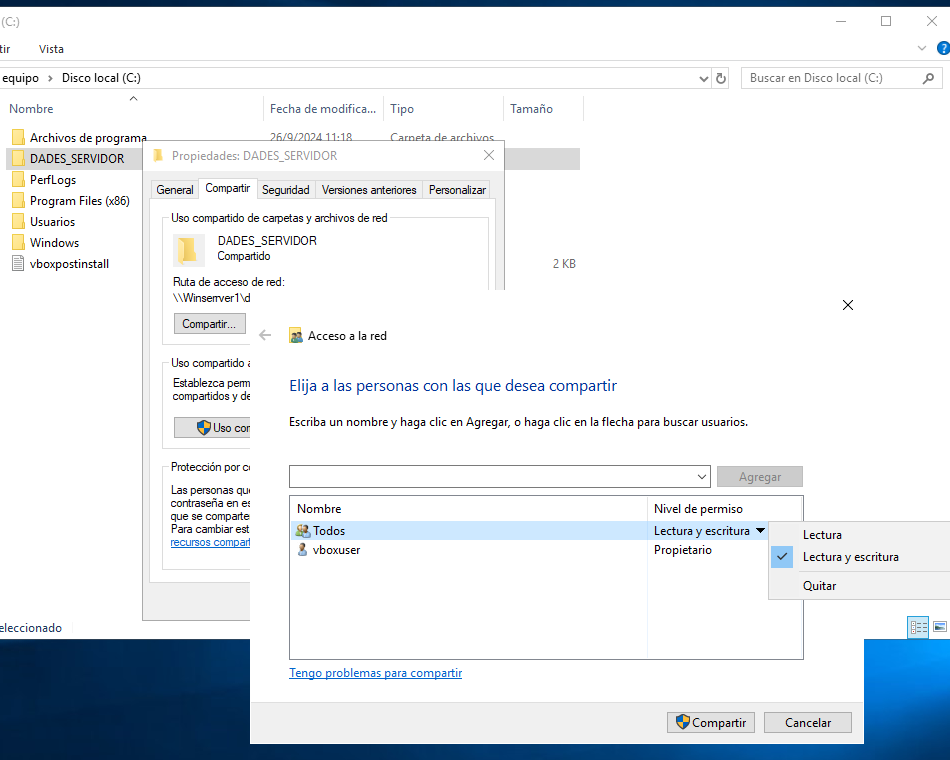
\includegraphics{png/ADDS/Compartir.png}
\caption{\emph{Compartició de carpeta}}
\end{figure}

Pondem limitar el nombre d'usuaris que hi poden accedir

\begin{figure}
\centering
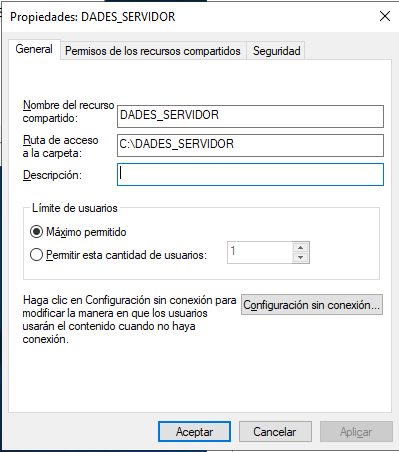
\includegraphics{png/ADDS/Compartir2.png}
\caption{\emph{Compartició de carpeta}}
\end{figure}

\begin{quote}
Nota:

La limitació d'usuaris és important per raons de seguretat (evitar
accesos desconeguts) però també per a mateniment: controlar si es queden
sessions sense tancar . Des de la consola del sistema de fitxers es
podrien expulsar. D'igual manera passaria amb els fitxers oberts.
\end{quote}

\subsection{6.2 Assignació o captura d'Unitat de
Xarxa}\label{assignaciuxf3-o-captura-dunitat-de-xarxa}

Ja ho hem vist anteriorment amb el Net use, però una vegaga funciona
correctament la els protocols que faciliten \emph{la compartició de
carpetes i impressores} i la \emph{detecció de la xarxa}, podem assignar
unitats a través del GUI buscant el recurs per la xarxa. Simplement amb
botó contrari \emph{Asignar unidad de red}. En reiniciar el client vorem
que continua (el mateix efecte que el /persistent:yes).

La forma en que es podrà automatitzar esta captura per a tots els
clients d'una xarxa la vorem més avant.

\subsection{6.3 Net use}\label{net-use}

Amb els comandaments \emph{net} podem, entre d'altres coses, assignar
també unitat de xarxa. Fins i tot quan no funcione la detecció de xarxes
(el problema de dependències tractat al punt 2.5 podem accedir a les
carpetes compartides a través de la xarxa fent ús dels comandaments
\emph{Net use}. Net use estableix una connexió directa basad en el
protocol SMB (Samba) i no usa els altres protocls al·ludits al punt 2.5.

\emph{Win + R:cmd}

\begin{Shaded}
\begin{Highlighting}[]
\NormalTok{net use F: \textbackslash{}\textbackslash{}WinServ1\textbackslash{}Dades2024 }\AttributeTok{/persistent:}\NormalTok{yes}
\end{Highlighting}
\end{Shaded}

Per veure totes les Unitat de xarxa ( ``lletres'') assignades

\begin{Shaded}
\begin{Highlighting}[]
\NormalTok{net use}
\end{Highlighting}
\end{Shaded}

Per eliminar-ne alguna

\begin{Shaded}
\begin{Highlighting}[]
\NormalTok{net use f: }\AttributeTok{/delete}
\end{Highlighting}
\end{Shaded}

\section{\texorpdfstring{7 Consola del sistema de fitxers
\emph{fsmgmt.msc}}{7 Consola del sistema de fitxers fsmgmt.msc}}\label{consola-del-sistema-de-fitxers-fsmgmt.msc}

La consola \emph{fsmgmt.msc} ens permet

\begin{itemize}
\tightlist
\item
  Tancar fitxers oberts en la xarxa
\item
  Veure els usuaris de xarxa que estan accedint-hi (sesiones)
\item
  Veure els recursos compartits amb el nom que es comparteixen. Si acaba
  amb \$ són ocults.
\end{itemize}

\begin{figure}
\centering
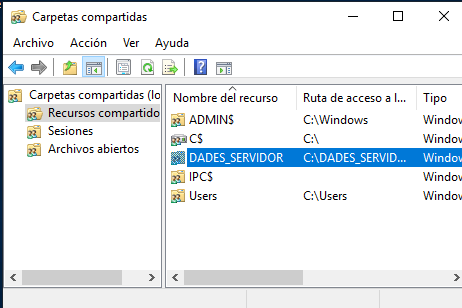
\includegraphics{png/ADDS/fsmgmt.png}
\caption{\emph{Consola de sistema de fitxers}}
\end{figure}

\section{8 Nota final sobre els prototocols en Windows
Server}\label{nota-final-sobre-els-prototocols-en-windows-server}

\textbf{Protocols}

La detecció de xarxes en Windows es basa en una combinació de protocols
(LLMNR, NetBIOS, SSDP) i serveis com. Tenim, per tant, unes
``dependències''. L'Explorador de equipos En canvi, el comandament
\textbf{net use} usa el protocolo \textbf{SMB Samba} per establiis una
\textbf{conexió directa} con el recurs compartit. També hem vist que
podem usar el \textbf{ICMP4} fent un ping.

\textbf{Com a servicis}

Per una banda veiem que podem habilitar-los com a serveis i, una vegada
habilitats, iniciar-los o apagar-los ( també inici automàtic).
\emph{Wind +R : services.msc}

\textbf{Firewall} El Firewall no sols pot bloquejar ``apliacions'' com
la \emph{detecció de xarxa} o \emph{compartició de fitxers i
impressores} que hem vist. També ens permet establir regles d'entrada o
eixida per a cadascun del protocols.

\begin{figure}
\centering
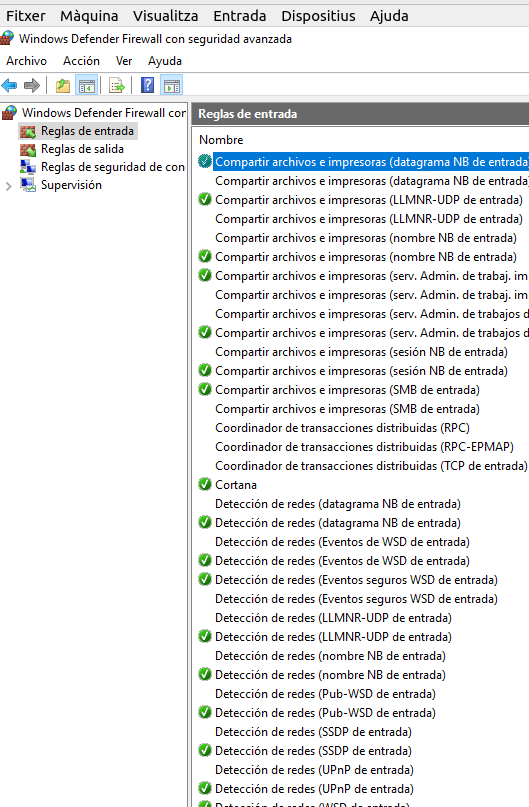
\includegraphics{png/ADDS/ExemplesEnFirewall.png}
\caption{\emph{Vista del Firewall}}
\end{figure}

\end{document}
